\bigskip

\item The equation $y = x^3 + 2 x^2 - 5x - 6$ is represented by which graph?

% \resizebox{5in}{!}{\includegraphics{SVC.01.06.080.ps}}
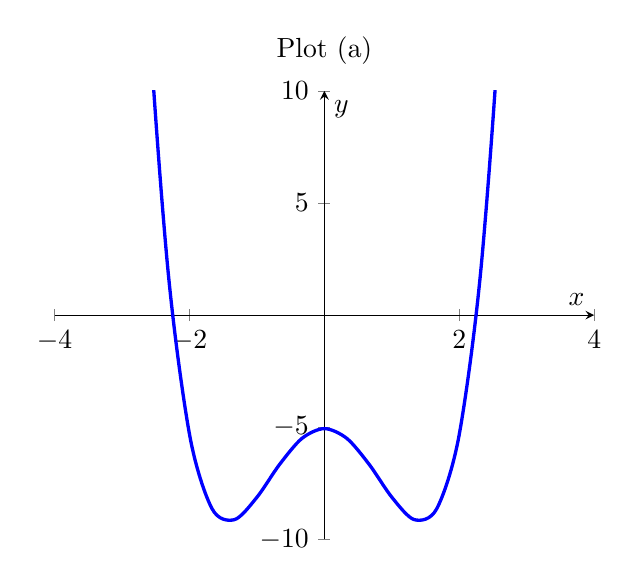
\begin{tikzpicture}
        \begin{axis}[axis lines=center, xlabel={$x$}, ylabel={$y$}, xmin=-4, xmax=4,
                ymin=-10, ymax=10, title={Plot (a)}]
                \addplot[color=blue, very thick, domain=-4:4, smooth]
                {(x-2.25)*(x+2.25)*(x^2+1)};
            \end{axis}
        \end{tikzpicture}
    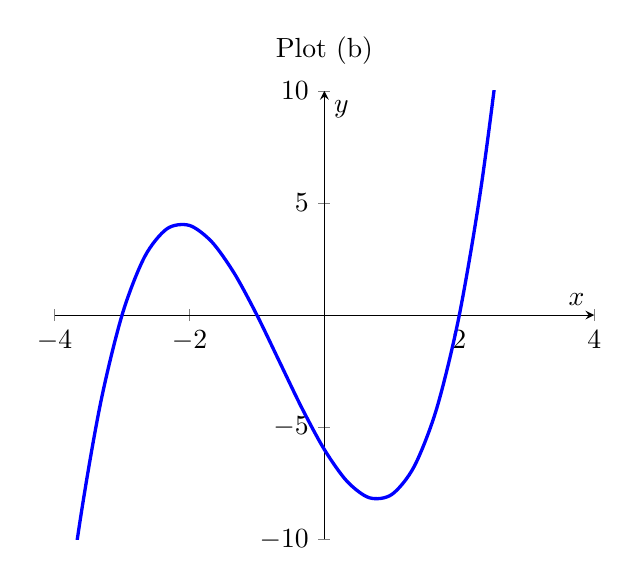
\begin{tikzpicture}
        \begin{axis}[axis lines=center, xlabel={$x$}, ylabel={$y$}, xmin=-4, xmax=4,
                ymin=-10, ymax=10, title={Plot (b)}]
                \addplot[color=blue, very thick, domain=-4:4, smooth]
                {x^3+2*x^2-5*x-6};
            \end{axis}
        \end{tikzpicture}\\
    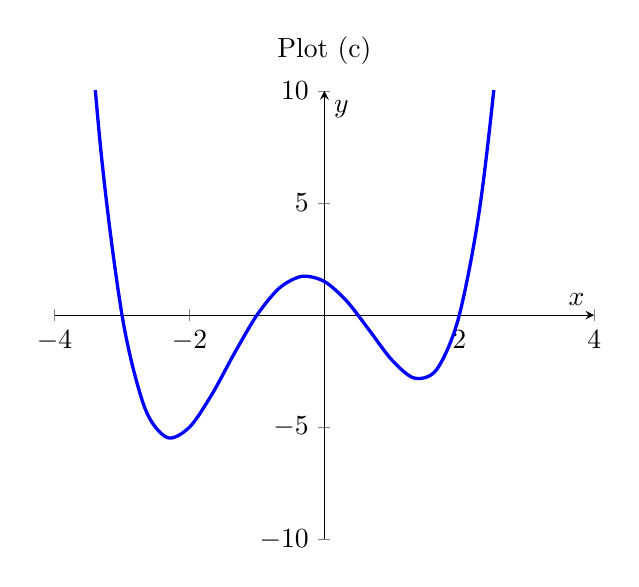
\begin{tikzpicture}
        \begin{axis}[axis lines=center, xlabel={$x$}, ylabel={$y$}, xmin=-4, xmax=4,
                ymin=-10, ymax=10, title={Plot (c)}]
                \addplot[color=blue, very thick, domain=-4:4, smooth]
                {0.5*(x+3)*(x+1)*(x-0.5)*(x-2)};
            \end{axis}
        \end{tikzpicture}
    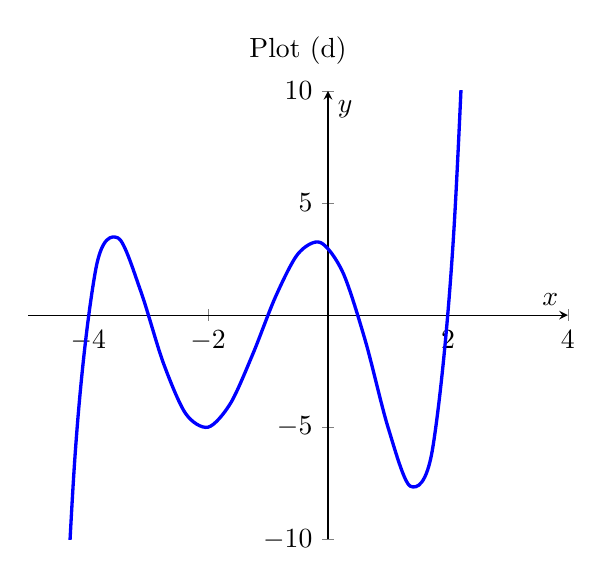
\begin{tikzpicture}
        \begin{axis}[axis lines=center, xlabel={$x$}, ylabel={$y$}, xmin=-5, xmax=4,
                ymin=-10, ymax=10, title={Plot (d)}]
                \addplot[color=blue, very thick, domain=-5:4, smooth]
                {0.25*(x+4)*(x+3)*(x+1)*(x-0.5)*(x-2)};
            \end{axis}
        \end{tikzpicture}


% ConcepTests - to accompany Calculus 4th Edition, Hughes-Hallet et al. John Wiley \& Sons.
